% Created 2019-09-26 Thu 00:15
% Intended LaTeX compiler: pdflatex
\documentclass[10pt,t]{beamer}
\usepackage[utf8]{inputenc}
\usepackage[T1]{fontenc}
\usepackage{graphicx}
\usepackage{grffile}
\usepackage{longtable}
\usepackage{wrapfig}
\usepackage{rotating}
\usepackage{amsmath}
\usepackage{textcomp}
\usepackage{amssymb}
\usepackage{capt-of}
\usepackage{hyperref}
\usetheme{default}
\author{L. Larrabee Strow}
\date{\today}
\title{\large AIRS Derived CO2 Zonal Anomalies over Ocean}
\subtitle{\footnotesize{AIRS Science Team Meeting}}
\date{\vspace{0.1in}\footnotesize{September 26, 2019\vfill}}
\author{L. Larrabee Strow\inst{1,2} and Sergio De Souza-Machado, UMBC\inst{1,2}}
\institute[UMBC]{\inst{1} UMBC Physics Dept. \and \inst{2}UMBC JCET}
\input beamer_setup
\usetheme{metropolis}
\metroset{titleformat title=allcaps}
\renewcommand{\UrlFont}{\small\tt}
\renewcommand*{\UrlFont}{\footnotesize}
\tolerance=1000
\RequirePackage{fancyvrb}
\DefineVerbatimEnvironment{verbatim}{Verbatim}{fontsize=\footnotesize}
\hypersetup{
 pdfauthor={L. Larrabee Strow},
 pdftitle={\large AIRS Derived CO2 Zonal Anomalies over Ocean},
 pdfkeywords={},
 pdfsubject={},
 pdfcreator={Emacs 26.1 (Org mode 9.2)}, 
 pdflang={English}}
\begin{document}

\maketitle
\addtobeamertemplate{block begin}{
  \setlength{\parsep}{0pt}
  \setlength{\topsep}{3pt plus 2pt minus 2.5pt}
  \setlength{\itemsep}{0pt plus 0pt minus 2pt}
  \setlength{\partopsep}{2pt}
}

\begin{frame}[label={sec:orgf59adbe}]{Introduction}
\begin{itemize}
\item How to AIRS growth rate anomalies compare to OCO
\item OCO is column, AIRS is broad kernel around 400 mbar, little surface contribution
\item OCO is quite heavily constrained over ocean in the S. Hemisphere
\item Why: AIRS S. Hemisphere anomalies grew during 2015 ENSO before the N. Hemisphere anomalies.  Doesn't seem right?
\item Either very interesting, or, more likely, good way to investigate ultimate accuracy of AIRS \cd anomalies.
\end{itemize}
\end{frame}

\begin{frame}[label={sec:org0403de0}]{\cd Anomaly Fit for 20\textdegree{} N. (MLO)}
\vspace{-0.3in}
\begin{columns}
\begin{column}{0.55\columnwidth}
\begin{block}{\footnotesize Fitting Trick}
\begin{center}
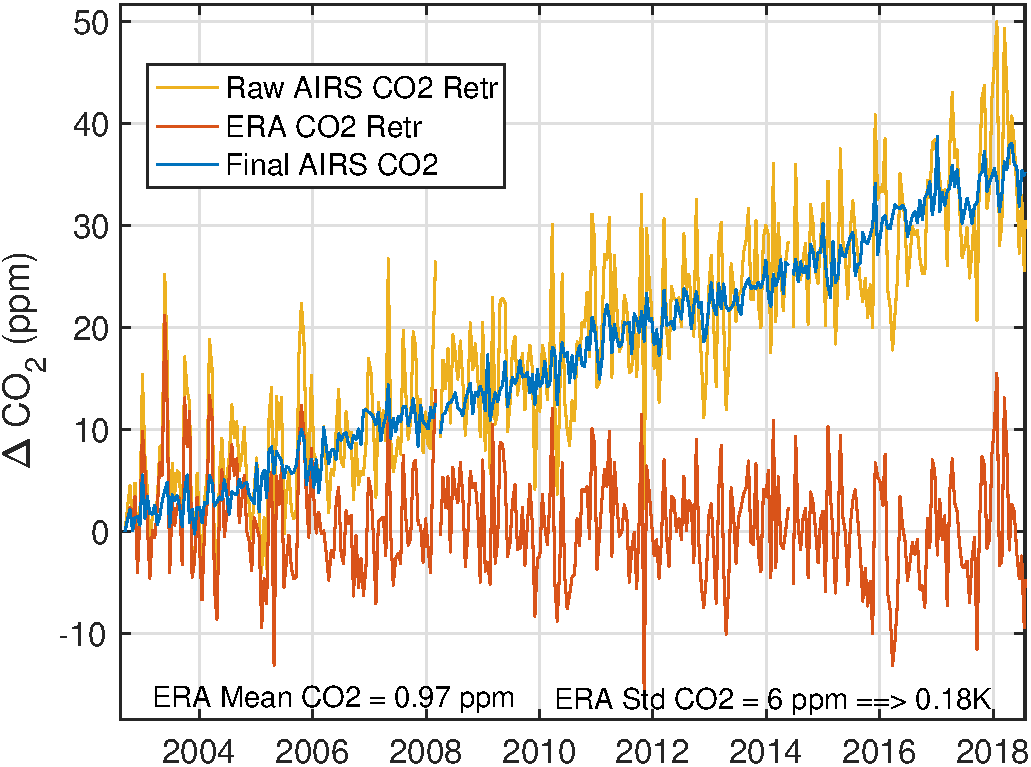
\includegraphics[width=\linewidth]{./Figs/Pdf/raw_co2_vs_era_co2_example_lati28_mlo_lat.pdf}
\end{center}
\end{block}
\end{column}

\begin{column}{0.55\columnwidth}
\begin{block}{\footnotesize Fitted \cd Anomalies}
\begin{center}
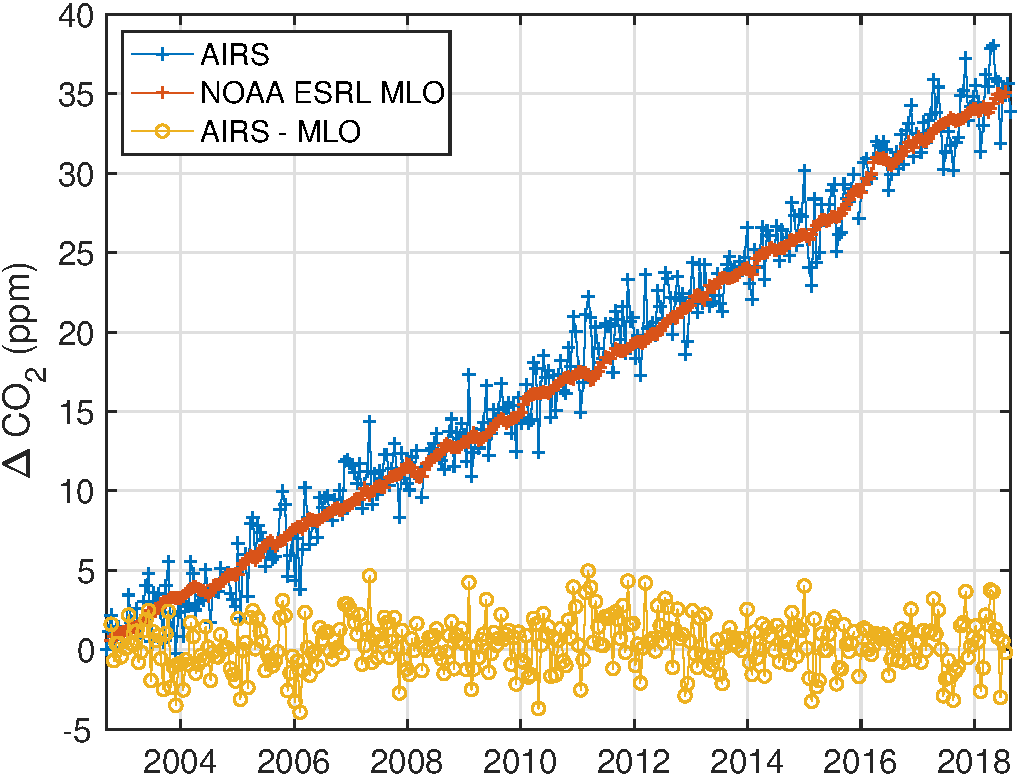
\includegraphics[width=\linewidth]{./Figs/Pdf/co2_airs_vs_mlo.pdf}
\end{center}
\end{block}
\end{column}
\end{columns}

\begin{footnotesize}
\begin{itemize}
\item ERA simulations done per footprint
\item Fit ERA simulation for \cd
\item Removes co-linearity? and lowers "noise"
\item Possible approach for Level 2 \cd retrievals?
\end{itemize}
\end{footnotesize}
\end{frame}

\begin{frame}[label={sec:org68f4f5f}]{\cd Anomaly Converted to B(T) Trends}
\begin{center}
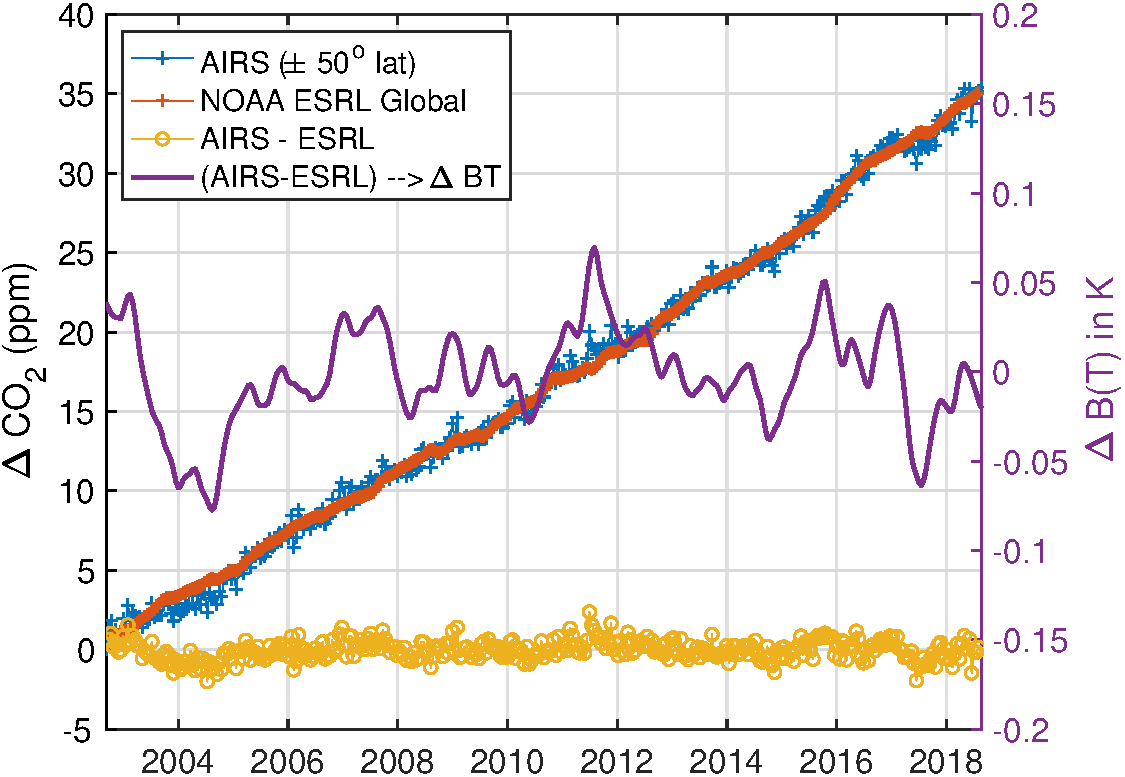
\includegraphics[width=0.7\linewidth]{./Figs/Pdf/co2_airs_vs_esrl_global_with_dbt.pdf}
\end{center}

\vspace{-0.1in}
\begin{footnotesize}
\begin{itemize}
\item Mean AIRS-ESRL \cd = 0.035 \textpm{} 0.032  pppm (1\(\sigma\) standard error)
\item Mean AIRS-ESRL in BT Units = +0.0026K \textpm{} 0.0023K (1\(\sigma\) standard error)
\item Sampling and ESRL errors hard to characterize
\end{itemize}
\end{footnotesize}
\end{frame}

\begin{frame}[label={sec:orgf269d09}]{\cd Trends and Growth Anomalies}
\vspace{-0.35in}
\begin{columns}
\begin{column}{0.5\columnwidth}
\begin{block}{\footnotesize Growth Rates}
\vspace{-0.1in}
\begin{center}
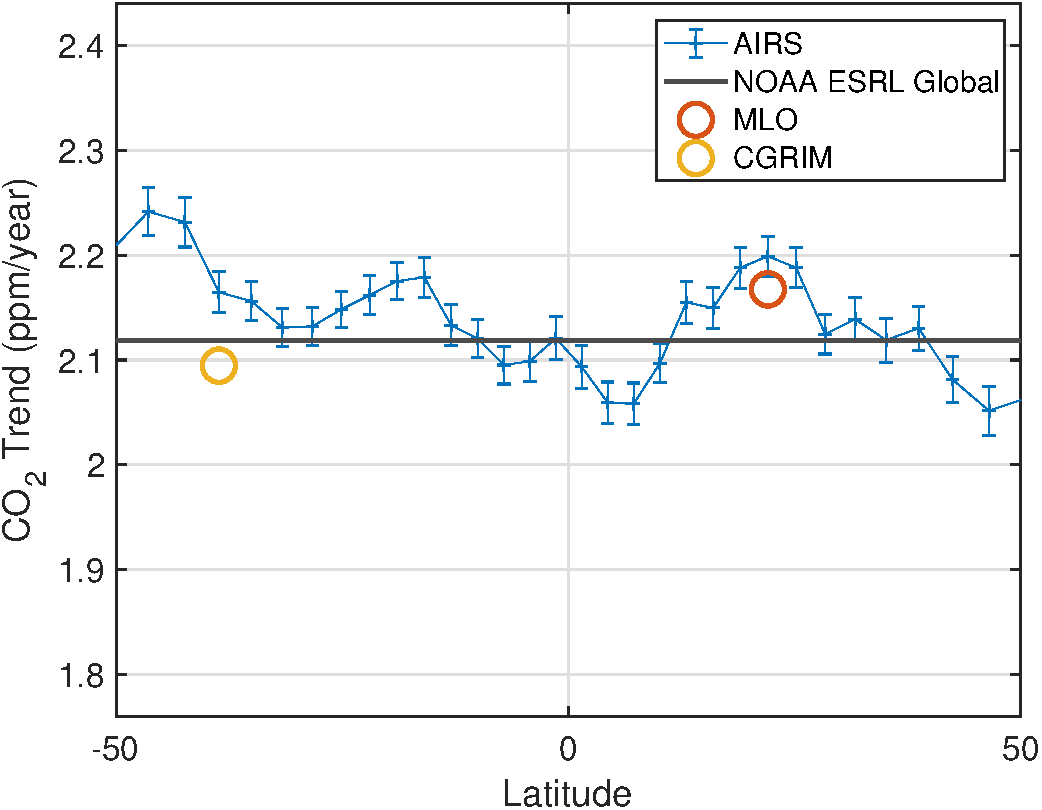
\includegraphics[width=0.9\linewidth]{./Figs/Pdf/co2_growth_vs_lat.pdf}
\end{center}
\end{block}
\end{column}

\begin{column}{0.5\columnwidth}
\begin{block}{\footnotesize Growth Rate Anomaly}
\vspace{-0.1in}
\begin{center}
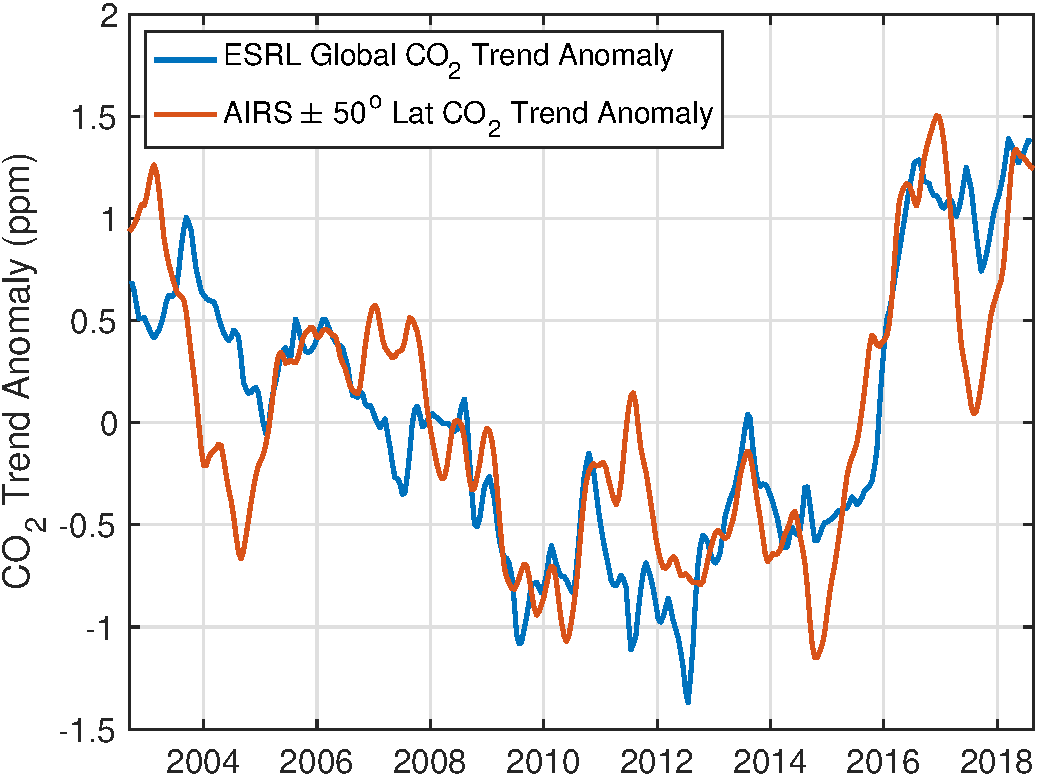
\includegraphics[width=0.9\linewidth]{./Figs/Pdf/co2_airs_vs_esrl_global_growth_anom.pdf}
\end{center}
\end{block}
\end{column}
\end{columns}

\vspace{-0.2in}

\begin{columns}
\begin{column}{0.5\columnwidth}
\begin{block}{\footnotesize Zonal Anomalies}
\vspace{-0.1in}
\begin{center}
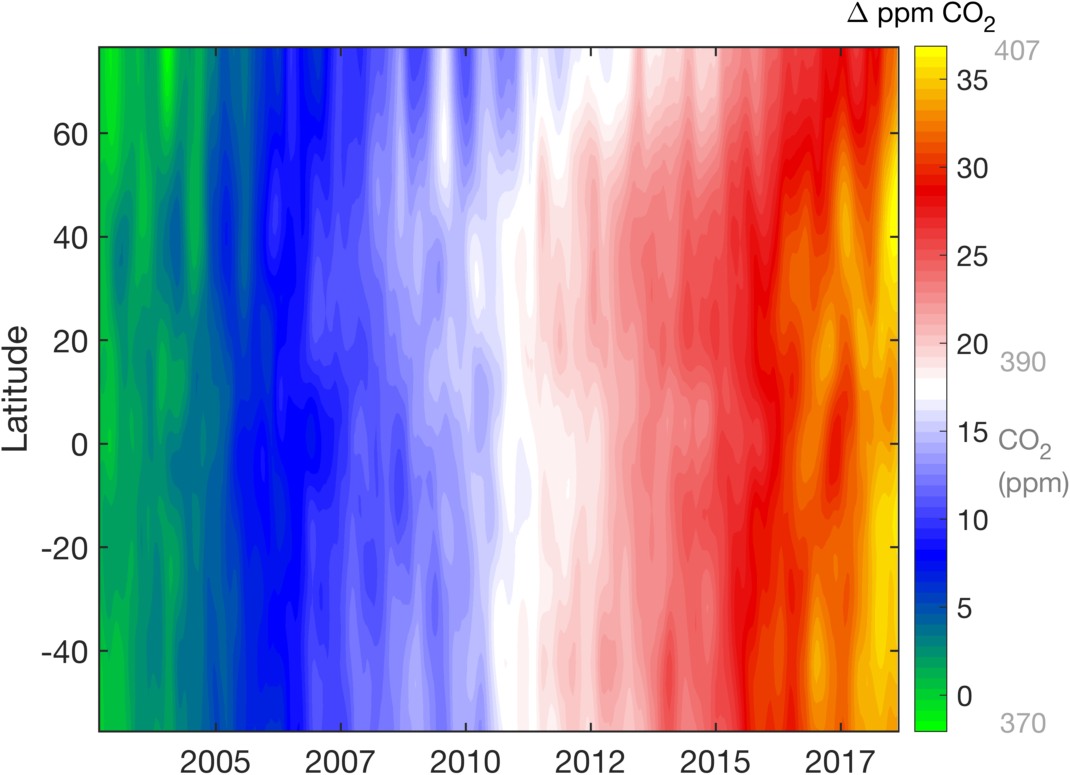
\includegraphics[width=0.9\linewidth]{./Figs/Png/co2_anom_image_lat_vs_time.png}
\end{center}
\end{block}
\end{column}

\begin{column}{0.5\columnwidth}
\begin{block}{}
\vspace{-0.2in}
\begin{footnotesize}
\begin{itemize}
\item Growth rate anomaly accuracy very encouraging.
\item AIRS - Avg(MLO + CGRIM) growth rate difference: -0.0056K/year in BT units
\item MLO, CGRIM growth rate uncertainty from ESRL \textasciitilde{}0.0051K/year
\end{itemize}
\end{footnotesize}
\end{block}
\end{column}
\end{columns}
\end{frame}


\begin{frame}[label={sec:orgff8737e}]{Zonal \cd Growth Anomalies}
\vspace{-0.1in}

\begin{center}
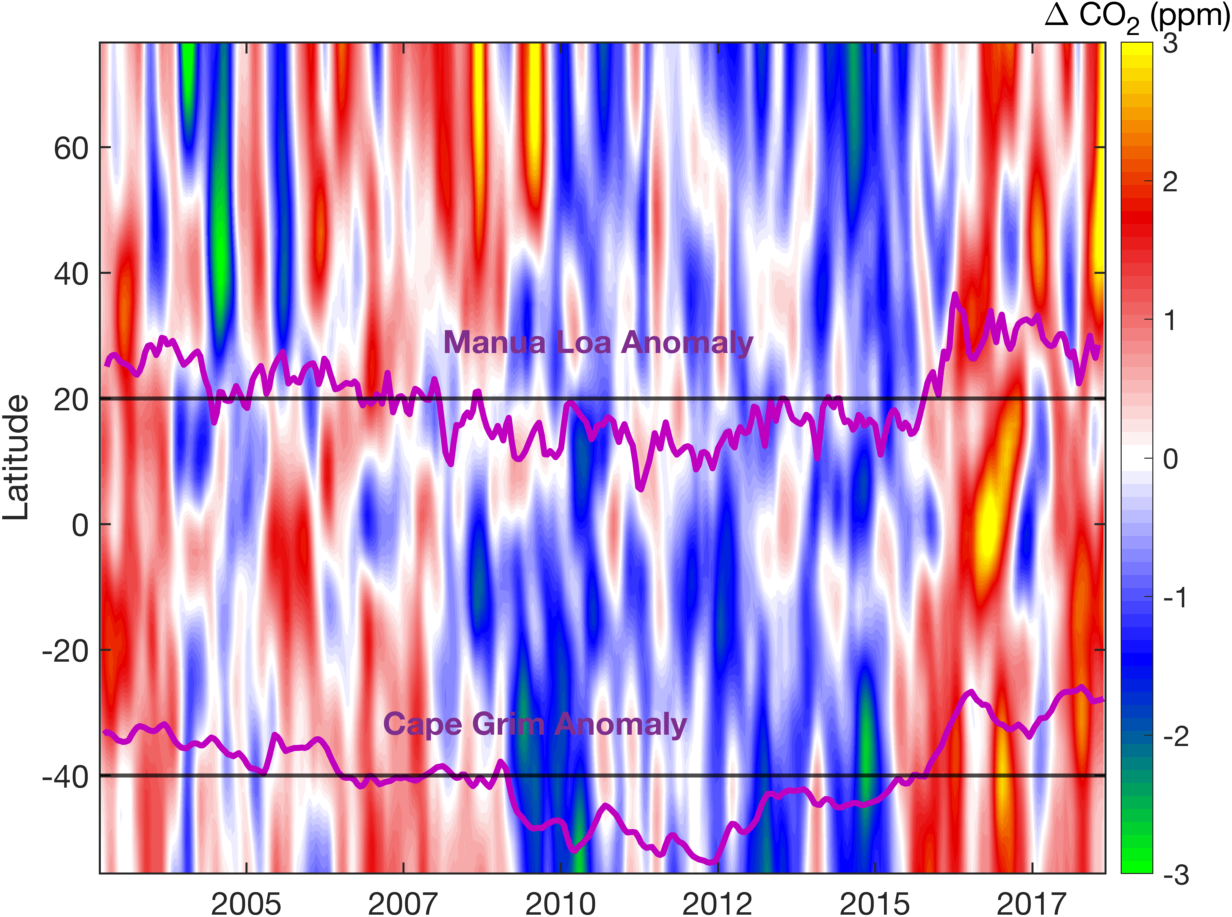
\includegraphics[width=0.65\linewidth]{./Figs/Png/co2_anomaly_image_fancy2_corrected.png}
\end{center}

\begin{footnotesize}
\begin{itemize}
\item Growth rate anomaly = (\cd anomaly - \cd average growth rate)
\item Magenta are ESRL MLO and Cape Grim \cd growth rate anomalies
\item \cd color scale is equivalent to max \textpm{} 0.09K in BT units
\item What is real?  Smoothing may be an issue.
\item 2015 ENSO effects very clear
\end{itemize}
\end{footnotesize}
\end{frame}

\begin{frame}[label={sec:org9c5731f}]{Global Trend Anomalies: ESRL, AIRS, OCO-2 (ocean)}
\vspace{-0.1in}
\begin{center}
\includegraphics[width=0.75\linewidth]{./oco/esrl_airs_oco_global_trend_anomaly.pdf}
\end{center}
\small
\begin{itemize}
\item At this level AIRS and OCO agree better than ESRL for 2015 ENSO
\item OCO smaller ENSO shift than ESRL
\item Still very clear AIRS has a Nov. 2003 shutdown problem
\end{itemize}
\end{frame}

\begin{frame}[label={sec:org6d2addd}]{OCO Zonal Growth Anomaies}
\begin{columns}
\begin{column}{0.55\columnwidth}
\begin{block}{OCO Anomalies}
\begin{center}
\includegraphics[width=0.9\linewidth]{./oco/co2_anomaly_OCO_orig_not_converted_to_airs_linear_rate.png}
\end{center}
\end{block}
\end{column}

\begin{column}{0.55\columnwidth}
\begin{block}{Adjust OCO to AIRS Anomaly Start}
\begin{center}
\includegraphics[width=0.9\linewidth]{./oco/first_oco_anomaly_airs_slopes_same_colorscale.png}
\end{center}
\end{block}
\end{column}
\end{columns}

\begin{itemize}
\item Need to convert OCO anomalies to zero in Sept. 2002 for comparison to AIRS
\end{itemize}
\end{frame}

\begin{frame}[label={sec:orgc43ac05}]{Intercompare AIRS and OCO Anomalies}
\vspace{-0.1in}

\begin{columns}
\begin{column}{0.55\columnwidth}
\begin{block}{\footnotesize AIRS Growth Anomalies, OCO Time Frame}
\begin{center}
\includegraphics[width=\linewidth]{./oco/co2_anomaly_image_fancy2_corrected_z1.png}
\end{center}
\end{block}
\end{column}

\begin{column}{0.55\columnwidth}
\begin{block}{\footnotesize OCO Growth Anomalies}
\begin{center}
\includegraphics[width=\linewidth]{./oco/co2_anomaly_OCO_image_fancy2_z1.png}
\end{center}
\end{block}
\end{column}
\end{columns}

\small 
\begin{itemize}
\item Notice high OCO at lowest latitudes
\item Why is AIRS ENSO higher in tropics?  Transport from N.H.?
\item More work needed to understand -40 deg. lat timing of \cd anomaly
\item Compare to OCO Anomaly on previous slide
\end{itemize}
\end{frame}


\begin{frame}[label={sec:orgec7a808}]{OCO A-Priori for Ocean, 400 mbar}
\begin{columns}
\begin{column}{0.55\columnwidth}
\begin{block}{OCO \cd A-Priori 400 mbar}
\begin{center}
\includegraphics[width=0.9\linewidth]{./oco/oco_co2_apriori_400mbar.pdf}
\end{center}
\end{block}
\end{column}

\begin{column}{0.55\columnwidth}
\begin{block}{OCO \cd A-Priori Std}
\begin{center}
\includegraphics[width=0.9\linewidth]{./oco/oco_co2_apriori_std_400mbar.pdf}
\end{center}
\end{block}
\end{column}
\end{columns}

\small OCO 400 mbar (and much of ocean profile) a-priori uncertainty is \textasciitilde{}1 ppm
\end{frame}

\begin{frame}[label={sec:org20196fa}]{Conclusions}
\begin{itemize}
\item Need to develop a gridded clear AIRS L1c subset
\item Present subset is highly non-uniform spatially
\begin{itemize}
\item However, fairly uniform near Cape-Grim at -40 deg
\end{itemize}
\item Use these results to further understand ultimate accuracy of AIRS \cd retrievals
\end{itemize}
\end{frame}
\end{document}